\documentclass[a4paper,12pt]{article}
\usepackage{amsfonts}
\usepackage{amsmath}
\usepackage{graphicx}
\usepackage{amssymb}
\usepackage{array}
\usepackage[round]{natbib}
\usepackage{booktabs}
\usepackage{floatpag}
\usepackage[hmargin=2.5cm,vmargin=3cm]{geometry}
\usepackage{setspace}
\usepackage{chngcntr}
\usepackage{verbatim}
\usepackage{multirow}
\usepackage{url}
\usepackage{doi}
\usepackage{hyperref}
\usepackage{xcolor}
\hypersetup{
    colorlinks,
    linkcolor={blue!50!black},
    citecolor={blue!50!black},
    urlcolor={blue!80!black}
}

\usepackage[gen]{eurosym}
\floatpagestyle{plain}
\newcolumntype{H}{>{\setbox0=\hbox\bgroup}c<{\egroup}@{}}
\renewcommand{\floatpagefraction}{0.95}
\setstretch{1.5}
\newcommand{\pathTables}{tables/}
\newcommand{\pathFigures}{}
\newcommand{\pathA}{}
\newcommand{\pathB}{}
\newcommand{\pathC}{}
\begin{document}
\pagenumbering{gobble}

\author{Marek Jaroci\'nski\thanks{%
European Central Bank DG-Research, email: marek.jarocinski@ecb.europa.eu}}
\title{Online Appendix to ``Central Bank Information Effects and Transatlantic Spillovers''}
\date{\today}
\maketitle

\appendix

\renewcommand{\thesection}{Appendix \Alph{section}}
\renewcommand{\thesubsection}{\Alph{section}.\arabic{subsection}}
\counterwithin{equation}{section}
\renewcommand{\theequation}{\Alph{section}.\arabic{equation}}
\counterwithin{figure}{section}
\renewcommand{\thefigure}{\Alph{section}.\arabic{figure}}
\counterwithin{table}{section}
\renewcommand{\thetable}{\Alph{section}.\arabic{table}}

\renewcommand{\pathTables}{../workm_lp/}

\section{Data}


\subsection{High-frequency financial data}

\begin{itemize}
\item
\textbf{ECB interest rate surprise} - The first principal component of the Monetary Event window changes
in overnight index swaps (OIS) with maturities 1-, 3-, 6-months and 1-year (Identifiers: OIS1M, OIS3M, OIS6M, OIS1Y).\footnote{\label{footnote:pc}Prior to computing the first principal component the variables are rescaled by their standard deviations. The variables are not demeaned, to ensure
that when all variables are equal to zero the first principal component also equals zero. 
This first principal component is the linear combination of the rescaled variables that has
the maximum second moment (not the maximum variance).}
\emph{Source:} EA-MPD of \cite{Altavilla_etal_2019}. The Monetary Event window starts 15 minutes
before the press release and ends 15 minutes after the end of the press conference whenever there is one. 
The first principal component is rescaled so that its variance equals that of
the 1 year OIS rate changes in the Monetary Event window.
\item
\textbf{ECB stock price surprise} - 
Euro Stoxx 50 index change in the Monetary Event window in percentage points. Identifier: STOXX50E. \emph{Source:} EA-MPD of \cite{Altavilla_etal_2019}.
\item
\textbf{Fed interest rate surprise} - 
The first principal component of the Monetary Event Window changes in 
the current-month and three-month-ahead federal
funds futures contracts and changes in the second, third, and fourth eurodollar futures contracts,
which have 1.5, 2.5, and 3.5 quarters to expiration on average (Identifiers: MP1, FF4, ED2, ED3, ED4).\footnote{See footnote \ref{footnote:pc}.} Surprises in the Monetary Event Window are obtained by adding up the surprise in the \emph{Press Release window} and the surprise in the \emph{Press Conference window}, whenever there is one. \emph{Sources:} Surprises in the Press Release window, starting 10 minutes before the press release and ending 20 minutes afterwards, come from the \cite{Gurkaynak_Sack_Swanson_2005a} database updated until June 2019 by \cite{Gurkaynak_Karasoy_Lee_2022} and available in their replication files at \url{http://www.bilkent.edu.tr/~refet/GKL_replication.zip}. Surprises in the Press Conference window, starting 10 minutes before the press conference and ending 15 minutes after the end of the press conference, come from the Thomson Reuters Tick History Database. See Section \ref{sec: Fed press conf} for more details on the surprises in the Press Conference window.
The first principal component is rescaled so that its variance equals that of
the changes in the fourth eurodollar futures contract in the Monetary Event window.
\item
\textbf{Fed stock price surprise} - 
S\&P500 index change in the Monetary Event window, in percentage points. Identifier: SP500. \emph{Source:} as above.
\end{itemize}


\begin{table}[!htbp]
\begin{center}
\caption{Summary statistics of the surprises}\label{tab: surprises summary stats}
\begin{tabular}{lccc} \toprule
 & Total interest rate & & Stock price \\
 &  surprise, $i^{Total}$ & & surprise, $s$ \\
\midrule
\emph{ECB surprises}\\
Mean (std. err.) & 0.14 (0.26) & & -8.43 (3.98) \\
Standard deviation & 4.14 & & 64.38 \\
Auto-correlation (P-value) & -0.08 (0.22) & & -0.05 (0.40) \\
Correlation ($i^{Total}$, $s$) & & -0.13 \\
Frequency of sign($i^{Total}$) $\ne$ sign($s$) & & 0.51 \\
N. of observations & & 261 \\
\midrule
\emph{Fed surprises}\\
Mean (std. err.) & -1.55 (0.54) & & 1.32 (5.49) \\
Standard deviation & 7.08 & & 71.81 \\
Auto-correlation (P-value) & 0.03 (0.66) & & -0.10 (0.21) \\
Correlation ($i^{Total},s$) & & -0.52 \\
Frequency of sign($i^{Total})\ne\,$sign($s$) & & 0.66 \\
N. of observations & & 171 \\
\bottomrule
\end{tabular}
\end{center}
\end{table}


\begin{table}[!htbp]
\begin{center}
\caption{Cross-correlations of Fed and ECB surprises}\label{tab: surprises correlations}
\begin{tabular}{p{7cm}ccccc} \toprule
 & \multicolumn{2}{c}{Total interest rate} &  \multicolumn{2}{c}{Stock price} & N. of\\
 &  \multicolumn{2}{c}{surprise, $i^{Total}$} &  \multicolumn{2}{c}{surprise, $s$} & pairs \\
\midrule
correlation between the Fed surprise and the most recent ECB surprise & -0.13 & (0.09) & 0.04 & (0.65) & 163 \\
correlation between the Fed surprise and the subsequent ECB surprise & -0.08 & (0.31) & 0.09 & (0.24) & 163 \\
\bottomrule
\end{tabular}
\end{center}\footnotesize
Note. P-values in parentheses. There are only 163 pairs of consecutive Fed and ECB surprises because sometimes there are two Fed surprises in a row without an ECB suprise in between.
\end{table}

\begin{figure}[!htbp]
\caption{Cumulated surprises}\label{fig: cumulated surprises}
\begin{center}
\begin{tabular}{cc}
\small Total interest rate surprises $i^{Total}$ & \small Stock price surprises $s$ \\
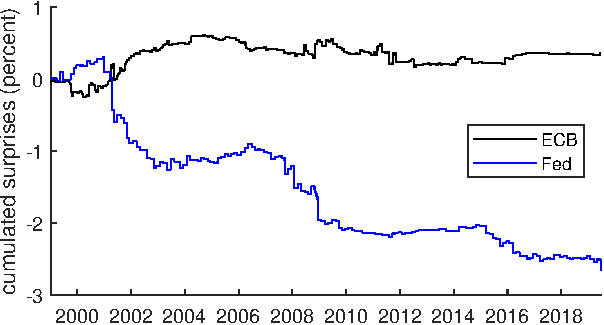
\includegraphics[width=0.47\textwidth]{figures/cumulated_surprises_pc1} &
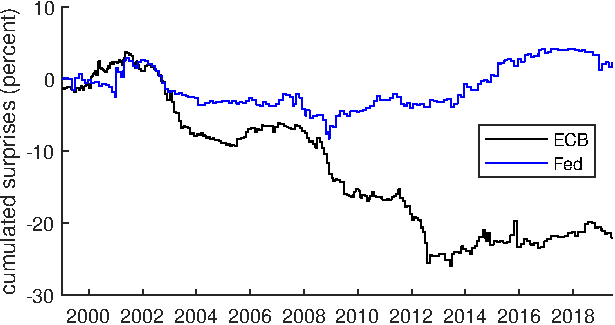
\includegraphics[width=0.47\textwidth]{figures/cumulated_surprises_stock}\\
\end{tabular}
\end{center}
\end{figure}

Table \ref{tab: surprises summary stats} reports the summary statistics of the Fed and ECB
interest rate and stock price surprises.
The ECB interest rate surprises are close to zero on average and have the standard deviation of about 4 basis points. The Fed interest rate surprises are negative on average, -1.55 basis point, and they have a larger standard deviation of 7 basis points. 
Contemporaneous interest rate and stock price surprises are negatively correlated.
For the Fed the correlation is as large as -0.52, suggesting that the monetary policy shocks
dominate, while for the ECB the correlation is only -0.13.
The autocorrelations of the surprises are negligible.
For simplicity I do not further purge these surprises from the component predictable by past information as purging makes little difference for subsequent inference. E.g. \cite{MirandaAgrippino_Ricco_2021} purge the surprises using one of the most comprehensive specifications, by regressing them on
their own lags and ten factors extracted from macroeconomics variables, but the unadjusted R-squared are below 0.1 (see their Table 3).
However, the correlations between the consecutive ECB and Fed surprises have not been explored previously.
Table \ref{tab: surprises correlations} shows that these correlations are small too. The first correlation of -0.13 is significant at the 10\% level but this correlation changes to 0.02
if one omits the large negative Fed surprise on April 18, 2001, which was preceded by a large positive ECB interest rate surprise on April 11.
Low correlations between consecutive shocks guarantee that we don't mistake the effects of domestic policy shocks for transatlantic spillovers.
Figure \ref{fig: cumulated surprises} plots the cumulated surprises of both central banks, interest rate surprises in the left panel and stock price surprises in the right panel. This figure shows that also at lower frequencies there is no systematic correlation between the Fed and ECB surprises.


\subsection{Macroeconomic news surprises}

\begin{itemize}
\item \textbf{Industry confidence} - European Commission Eurozone Industrial Confidence. Ticker: EUICEMU. \emph{Source:} Bloomberg. \emph{Units:} Index.
\item \textbf{Unemployment rate} - Eurostat Unemployment Eurozone SA. Ticker: UMRTEMU. \emph{Source:} Bloomberg. \emph{Units:} Percent.
\end{itemize}


\subsection{Daily financial data}\label{sec: daily data}

\begin{itemize}
\item
\textbf{1-year Bund yield, 10-year Bund yield} - \emph{Source:} Deutsche Bundesbank: Term structure of interest rates on listed Federal securities (method by Svensson) \url{https://www.bundesbank.de/dynamic/action/en/statistics/time-series-databases/time-series-databases/759784/759784?listId=www_skms_it03a}. \emph{Units:} percent. \emph{Transformation:} none.
\item
\textbf{1-year Treasury bond yield, 10-year Treasury bond yield} - Zero-coupon yield, Continuously Compounded. \emph{Source:} 
\url{https://www.federalreserve.gov/pubs/feds/2006/200628/200628abs.html} Identifiers: SVENY01, SVENY10. Reference: 
\cite{Gurkaynak_Sack_Wright_2007} \emph{Units}: percent. \emph{Transformation:} none.
\item
\textbf{S\&P500} - Standard and Poors 500 Composite Index \emph{Source:} Datastream. \emph{Units:} index. \emph{Transformation:} 100*log.
\item
\textbf{Euro Stoxx 50} - Dow Jones Euro Stoxx 50 EUR Price Index - \emph{Source:} Bloomberg. \emph{Units:} index. \emph{Transformation:} 100*log.
\item
\textbf{High yield corporate bond OAS (US)} - ICE BofA US High Yield Index Option-Adjusted Spread (OAS). US dollar denominated below investment grade
rated corporate debt publicly issued in the US domestic market. \emph{Source:} Fred, after Ice Data Indices, LLC. Identifier: bamlh0a0hym2. \emph{Units:} percent. \emph{Transformation:} none.
\item
\textbf{High yield corporate bond OAS (EA)} - ICE BofA Euro High Yield Index Option-Adjusted Spread (OAS). Euro denominated below
investment grade corporate debt publicly issued in the euro domestic  
or eurobond markets. \emph{Source:} Fred, after Ice Data Indices, LLC. Identifier: bamlhe00ehyioas. \emph{Units:} percent. \emph{Transformation:} none.
\item
\textbf{EUR per USD} - Exchange rate. \emph{Source:} ECB. \emph{Units:} Euros per one US dollar. \emph{Transformation:} 100*log.
\item
\textbf{Broad dollar ex EUR} - The Broad dollar index, calculated
by the Federal Reserve, is a trade-weighted exchange rate with respect to 26 most important trading partners by volume of the bilateral trade. I have recalculated this index taking the euro out of it. 
The construction of the Broad dollar index is explained in \cite{Beschwitz_etal_2019},
\url{https://www.federalreserve.gov/econres/notes/feds-notes/revisions-to-the-federal-reserve-dollar-indexes-20190115.htm}. The Broad dollar index back to 2006 was downloaded from the Federal Reserve website \url{https://www.federalreserve.gov/datadownload/Build.aspx?rel=H10}
and the euro's weights back to 2006 was downloaded from \url{https://www.federalreserve.gov/releases/h10/weights/default.htm}. The Broad dollar index and the euro's weights before 2006 were taken from the data appendix of \cite{Beschwitz_etal_2019}, \url{https://www.federalreserve.gov/econres/notes/ifdp-notes/IFDP_Note_Data_Appendix.xlsx}. I have removed the euro from the Broad dollar index and rescaled so that the weights of the remaining currencies add up to 1. 
\emph{Units:} index, foreign currency per one US dollar. \emph{Transformation:} 100*log.

More in detail, the Broad dollar index at time $t$ ($I_t$) is $I_t = I_{t-1} \prod_j^N (e_{j,t}/e_{j,t-1})^{w_{j,t}}$, where $e_{j,t}$ is the price of the dollar in terms of the foreign currency $j$ at time $t$ and $w_{j,t}$ is its weight \citep{Beschwitz_etal_2019}. Let the euro be the $N$th currency, let $\Delta i_t = \ln(I_t/I_{t-1})$ be the log change of the broad dollar index and let $c_{N,t} = w_{N,t}\ln (e_{N,t}/e_{N,t-1})$ be the euro's contribution to it. The log change of the Broad dollar ex EUR is computed as $\Delta i_t^\text{exEUR} = 1/(1-w_{N,t}) (\Delta i_t - c_{N,t})$.
\item
\textbf{S\&P500 Financials} - The S\&P 500 Financials comprises those companies included in the S\&P 500 that are classified as members of the GICS financials sector. Number of companies: 66. Total Return index. Ticker: SPTRFINL.
\emph{Source:} Bloomberg. \emph{Units:} index. \emph{Transformation:} 100*log.
\item
\textbf{S\&P500 Ex-Financials} - The S\&P 500 Ex-Financials is designed to provide broad market exposure except for members of the financials sector.
Number of companies: 439. Total Return index. Ticker: SPXXFIST.
\emph{Source:} Bloomberg. \emph{Units:} index. \emph{Transformation:} 100*log.
\item
\textbf{Wilshire US Small-Cap} - The Wilshire US Small-Cap is a float-adjusted, market capitalization-weighted index of the issues ranked between 750 and 2,500 by market capitalization of the Wilshire 5000 Total Market Index.
 Number of companies: 1745. Fred identifier: WILLSMLCAP.  \emph{Source}: Fred after Wilshire Associates. \emph{Units:} index. \emph{Transformation:} 100*log.
\item
\textbf{Wilshire US Large-Cap} - The Wilshire US Large-Cap Index is a float-adjusted, market capitalization-weighted index of the issues ranked above 750 by market capitalization of the Wilshire 5000 Total Market Index. Together, the components of the Wilshire US Large-Cap, Wilshire US Small-Cap Index and Wilshire US Micro-Cap Index comprise the Wilshire 5000 without gaps or overlaps. Number of companies: 750. Fred identifier: WILLLRGCAP. \emph{Source}: Fred after Wilshire Associates. \emph{Units:} index. \emph{Transformation:} 100*log.
\item
\textbf{Europe-exposed S\&P500, US-exposed S\&P500} - Based on Worldscope and Datastream.
The indices have a fixed composition and consist of 497 stocks that entered the S\&P500 for at least 40 quarters between 1998 and 2020.
For each of those 497 companies I obtain from Worldscope the share of sales in Europe in their total sales in the years 2000, 2005, 2010, 2015, 2020 and average it over time.
I take the daily data on prices and float-adjusted market capitalization from Datastream.
Then I construct a price index of these 497 stocks weighted by the float-adjusted market capitalization multiplied by the shares of European sales.
There are 252 companies with nonzero and non-missing average European sales shares, for 129 companies the share exceeds 10\% and for 90 companies the share exceeds 15\%.
I proceed analogously for the US-exposed companies.
There are 472 companies with nonzero and non-missing average US sales shares, for 175 companies the share exceeds 90\% and for 150 companies the share exceeds 95\%.
\emph{Units:} index. \emph{Transformation:} 100*log.
\item
\textbf{Fed funds futures next FOMC, Fed funds futures 3m, Fed funds futures 6m} - The rates implied by the 30-days federal funds futures after the Next FOMC meeting (based on the current month or next month futures, depending on the date of the next FOMC meeting), in 3-months and in 6-months. \emph{Source}: Haver. Identifiers: PNFP@DAILY, PFFN3P@DAILY and PFFN6P@DAILY \emph{Units:} percent. \emph{Transformation:} none.

\end{itemize}

\subsection{Monthly variables}

\begin{itemize}
\item
\textbf{Effective Federal Funds Rate} - daily average. \emph{Source:} Fred, after Board of Governors of the Federal Reserve System. Identifier: FEDFUNDS. \emph{Units:} Percent. \emph{Transformation:} none.
\item
\textbf{Shadow Federal Funds Rate (Wu-Xia)} - \cite{Wu_Xia_2016}. Downloaded
from \url{https://sites.google.com/view/jingcynthiawu/shadow-rates}.
\emph{Units:} Percent. \emph{Transformation:} none.
\item 
\textbf{Shadow Federal Funds Rate (Krippner)} - \cite{Krippner_2013,Krippner_2015}. Downloaded
from \url{https://www.ljkmfa.com/visitors/}.
\emph{Units:} Percent. \emph{Transformation:} none.
\item
\textbf{Broad euro} - Broad Effective Exchange Rate for Euro Area. \emph{Source:} Fred, after BIS.  Identifier NBXMBIS. \emph{Units:} index, foreign currency per one Euro. \emph{Transformation:} 100*log.
\item
\textbf{US Real GDP and GDP Deflator} - Interpolation by
\cite{Stock_Watson_2010} updated to 2019Q1. See the replication files for \cite{Jarocinski_Karadi_2020}. \emph{Transformation:} 100*log.
\item
\textbf{Euro area Real GDP and GDP Deflator} - Own interpolation following
\cite{Stock_Watson_2010}. See the replication files for \cite{Jarocinski_Karadi_2020}. \emph{Transformation:} 100*log.
\end{itemize}

The remaining monthly variables are the monthly averages of the daily variables discussed in \ref{sec: daily data}.

%%%%%%%%%%%%%%%%%%%%%%%%%%%%%%%%%%%%%%%%%%%%%%%%%%%%%%%%%%%%%%%%%%%%%%%%%%%%%%%%
%%%%%%%%%%%%%%%%%%%%%%%%%%%%%%%%%%%%%%%%%%%%%%%%%%%%%%%%%%%%%%%%%%%%%%%%%%%%%%%%
%%%%%%%%%%%%%%%%%%%%%%%%%%%%%%%%%%%%%%%%%%%%%%%%%%%%%%%%%%%%%%%%%%%%%%%%%%%%%%%%
\subsection{Fed announcement surprises in the press conference windows}\label{sec: Fed press conf}


\paragraph{The dates and times of the Fed press conferences.} 
The dates and times of the Fed post-FOMC meeting press conferences come from the Bloomberg Economic Calendar.
(See also \cite{Bodilsen_etal_2021} for a convenient summary table in their Online Appendix.)
The Fed started to hold press conferences after FOMC meetings on April 27, 2011. 
In the years 2011-2018 the press conferences were held after every other FOMC meeting
and since 2019 after every FOMC meeting.
In the years 2011-2012 the FOMC announcements were published at 12:30 and the press
conferences started at 14:15.
From 2013 onward the FOMC announcement was issued at 14:00 and the press conference started at 14:30.

\paragraph{Press Conference Window} 
I define a Press Conference Window that starts 10 minutes before the start of the press conference
and ends 75 minutes after the start of the press conference.
From 2013 onward the start of the Press Conference Window coincides with the end of the GSS FOMC press release window (the GSS window ends 20 minutes after the press release).
For the 8 press conferences held in the years 2011-2012 there is a gap 
between the end of the GSS window and the start of the Press Conference Window.
The press conferences last approximately one hour, so the Press Conference Window
ends approximately 15 minutes after the end of the press conference,
like in the \cite{Altavilla_etal_2019} dataset of the ECB surprises.


\paragraph{Summary statistics about press conference (PC) surprises.} 
The changes in the PC Window of the variables MP1, FF4, ED2, ED3, ED4 and SP500, defined in \cite{Gurkaynak_Sack_Swanson_2005a} are extracted from the Thomson Reuters Tick History database.
There are 36 press conferences between April 2011 and June 2019.
Figures \ref{fig: fed pr and pc}, \ref{fig: fed pr and pc 2}, \ref{fig: fed pr and pc 3} 
present the GSS surprises for all FOMC announcements from January 1999 until June 2019 along with the PC surprises available for 36 of these FOMC announcements.
Table \ref{tab: fed pr and pc} reports summary statistics computed on these 36 dates.
The PC variance share is defined as var($x^{PC}$)/(var($x^{PC}$)+var($x^{GSS}$)),
where $x^{PC}$ is the surprise in variable $x$ in the PC window and
$x^{GSS}$ is the surprise in variable $x$ in the press release window coming from the GSS database.
The table reports also the correlations between $x^{PC}$ and $x^{GSS}$ and their statistical significance.
First, on the press conference days the press conference windows
account for about one third of the variance of interest rate derivatives with maturities 3 months and more,
and less than that near-term futures MP1. For stock prices the press conference windows
account for 57\% of the variance.
Second, we can see in Figures \ref{fig: fed pr and pc}, \ref{fig: fed pr and pc 2}, \ref{fig: fed pr and pc 3} that in the press conference windows asset prices tend to move
in the same direction as in the preceding announcement windows. 
Indeed, Table \ref{tab: fed pr and pc}
shows that the correlations between the surprises in the two windows are positive, though not always statistically significant.
For the stock prices the correlation is 0.45 and highly significant.


\begin{table}[!htbp]
\begin{center}
\caption{Press conference (PC) surprises - variance shares and correlations with the GSS surprises}\label{tab: fed pr and pc}
\begin{tabular}{p{6cm}ccc}
\toprule
Variable & PC variance share & Corr($x^{PC},x^{GSS}$) & p-value \\
\midrule
MP1 & 0.04 & 0.15 & 0.41 \\
FF4 & 0.29 & 0.19 & 0.28 \\
ED2 & 0.38 & 0.34 & 0.04 \\
ED3 & 0.35 & 0.29 & 0.08 \\
ED4 & 0.29 & 0.23 & 0.17 \\
Total $i$ surprise (i.e. the 1st Principal Component of the above) & 0.31 & 0.29 & 0.09 \\
SP500 & 0.57 & 0.45 & 0.01 \\
\bottomrule
\end{tabular}
\end{center}\footnotesize
Note. The PC variance share of variable $x$ is defined as var($x^{PC}$)/(var($x^{PC}$)+var($x^{GSS}$)).
The p-value indicates the statistical significance of the correlation.
Both the variance shares and the correlations are computed over the 36 observations
with press conferences.
\end{table}


\renewcommand{\pathA}{../data/shocks/plots_pconf}
\begin{figure}[p]
\caption{Fed surprises in the Press Release and Press Conference windows}\label{fig: fed pr and pc}
\begin{center}
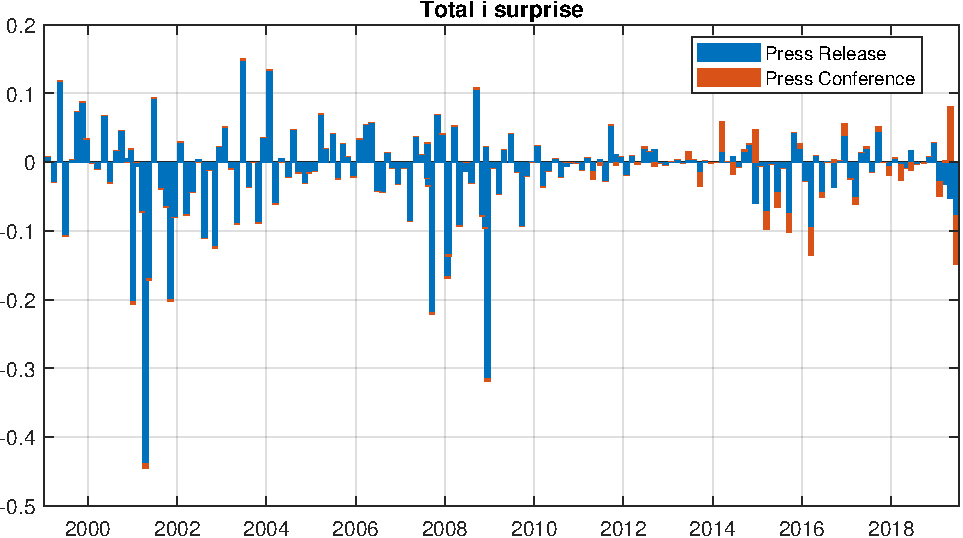
\includegraphics[width=0.7\textwidth]{\pathA/contrib_pr_pc_pc1ff1_pr}\\
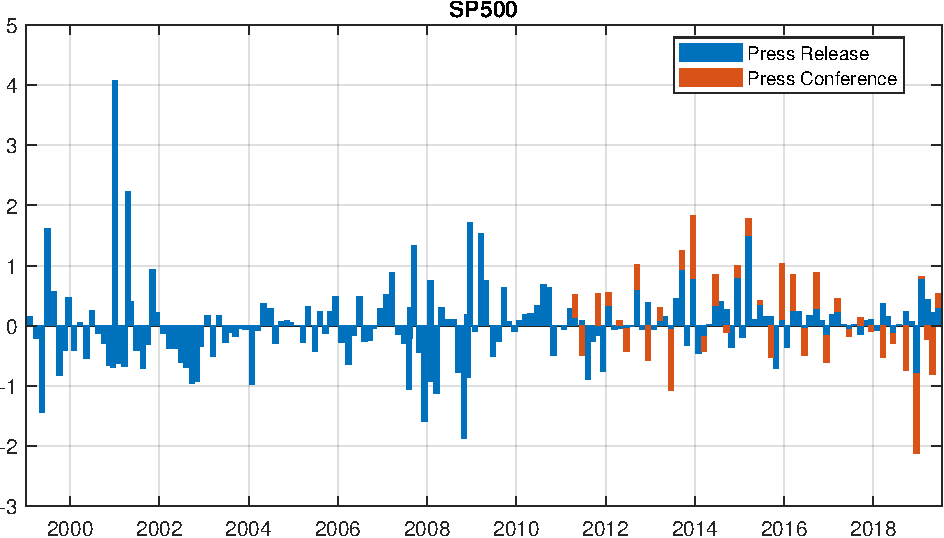
\includegraphics[width=0.7\textwidth]{\pathA/contrib_pr_pc_SP500}\\
\end{center}
\footnotesize Note. Blue bars show the surprises in the press release window, from GSS. Red bars show the surprises in the press conference window, from Thomson Reuters Tick History.
\end{figure}

\begin{figure}[p]
\caption{Fed surprises in the Press Release and Press Conference windows - continued}\label{fig: fed pr and pc 2}
\begin{center}
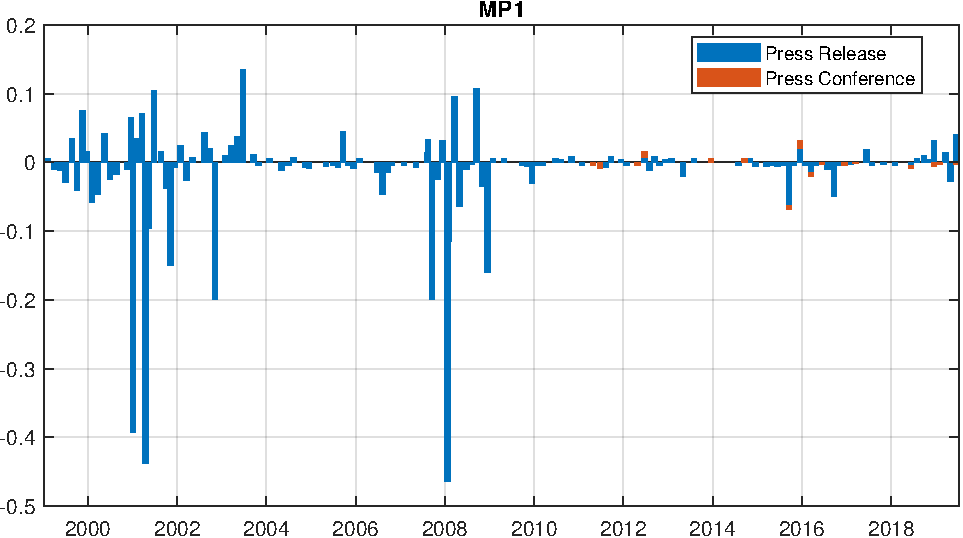
\includegraphics[width=0.7\textwidth]{\pathA/contrib_pr_pc_MP1}\\
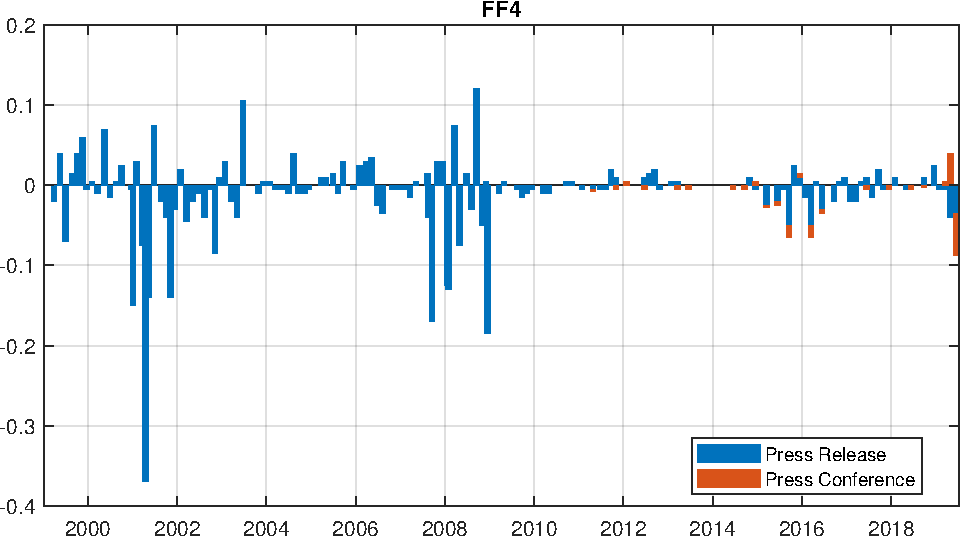
\includegraphics[width=0.7\textwidth]{\pathA/contrib_pr_pc_FF4}\\
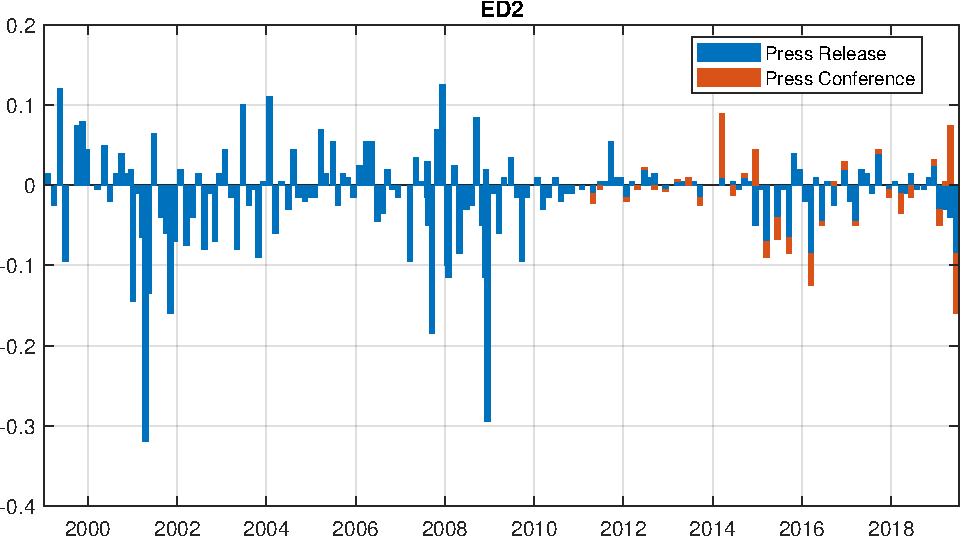
\includegraphics[width=0.7\textwidth]{\pathA/contrib_pr_pc_ED2}\\
\end{center}
\footnotesize Note. Blue bars show the surprises in the press release window, from GSS. Red bars show the surprises in the press conference window, from Thomson Reuters Tick History.
\end{figure}

\begin{figure}[p]
\caption{Fed surprises in the Press Release and Press Conference windows - continued}\label{fig: fed pr and pc 3}
\begin{center}
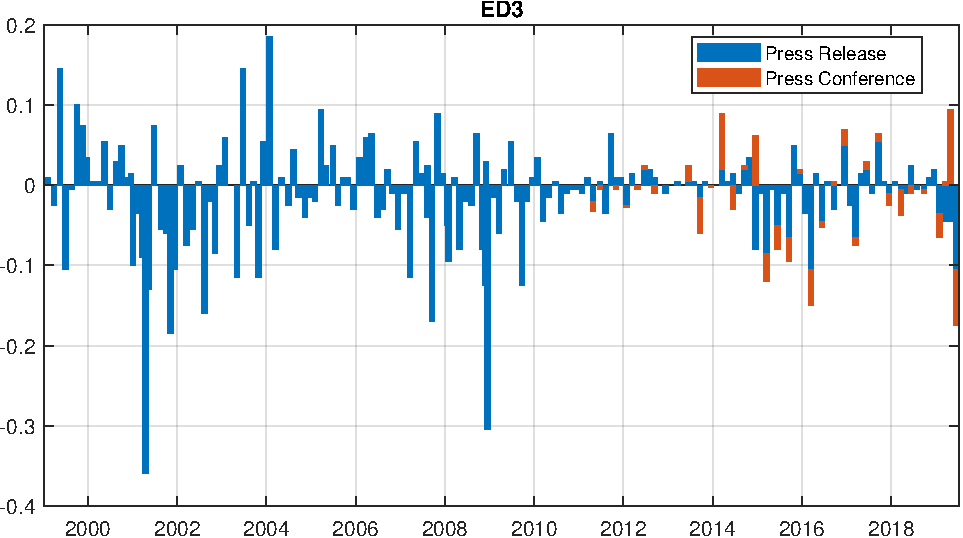
\includegraphics[width=0.7\textwidth]{\pathA/contrib_pr_pc_ED3}\\
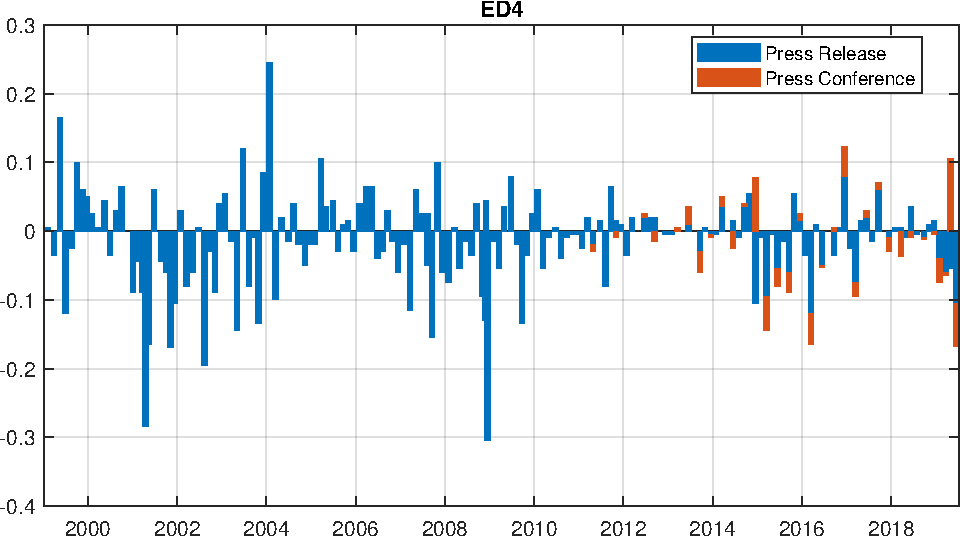
\includegraphics[width=0.7\textwidth]{\pathA/contrib_pr_pc_ED4}\\
\end{center}
\footnotesize Note. Blue bars show the surprises in the press release window, from GSS. Red bars show the surprises in the press conference window, from Thomson Reuters Tick History.
\end{figure}


\clearpage

%%%%%%%%%%%%%%%%%%%%%%%%%%%%%%%%%%%%%%%%%%%%%%%%%%%%%%%%%%%%%%%%%%%%%%%%%%%%%%%%
%%%%%%%%%%%%%%%%%%%%%%%%%%%%%%%%%%%%%%%%%%%%%%%%%%%%%%%%%%%%%%%%%%%%%%%%%%%%%%%%
%%%%%%%%%%%%%%%%%%%%%%%%%%%%%%%%%%%%%%%%%%%%%%%%%%%%%%%%%%%%%%%%%%%%%%%%%%%%%%%%
\section{Rotational sign restrictions}
\newcommand{\vsmp}{\frac{\operatorname{var}(i^{MP})}{\operatorname{var}(i^{Total})}}
\newcommand{\vscbi}{\frac{\operatorname{var}(i^{CBI})}{\operatorname{var}(i^{Total})}}

This section explains the details of rotational sign restrictions. Recall that the goal is to decompose the interest rate surprises into a sum of two orthogonal
components, such that the first one is associated with a negative
co-movement of the interest rate and stock price surprises and the second is associated with their positive co-movement.

Recall also that $i^{Total}$ is a vector of interest rate surprises, $s$ is a vector of stock price surprises, $i^{MP}$ is a vector of monetary policy shock proxies and $i^{CBI}$ is a vector of central bank information shock proxies. Each of the four vectors has length $T$, where $T$ is the number of central bank announcements in the dataset. Let $M=(i^{Total},s)$ be a $T \times 2$ matrix with columns $i^{Total}$ and $s$.
I decompose $M$ as
\begin{equation} M = UC,\quad  \text{where}\quad U=\left(i^{MP},i^{CBI}\right), \quad (i^{MP})'i^{CBI}=0 \quad \text{and}\quad
C=\begin{pmatrix}1&c_{MP}<0\\1&c_{CBI}>0\end{pmatrix}.\label{eq: rotational sign restrictions}
\end{equation}

The decomposition in (\ref{eq: rotational sign restrictions}) is not unique. There is a range of ``rotations'' of $U$ and $C$ that all satisfy the sign restrictions $c_{MP}<0$ and $c_{CBI}>0$. 

\subsection{Computing the decomposition}
$U$ and $C$ are computed as
\begin{equation}
U = QPD \quad \text{and} \quad C = D^{-1}P'R
\end{equation}
where the matrices $Q,P,D,R$ are obtained in three steps.

\bigskip
\noindent 1. \emph{Decompose $M$ into two orthogonal components} using the QR decomposition,
\begin{equation}
M = QR,\quad  \text{where}\quad Q'Q=\begin{pmatrix}1&0\\0&1\end{pmatrix}\quad \text{and}\quad
R=\begin{pmatrix}r_{11}>0&r_{12}\\0&r_{22}>0\end{pmatrix}.
\end{equation}
Note that in many software packages do not impose the normalization that the diagonal elements of $R$ are positive, in this case this has to be imposed ex post.

\bigskip
\noindent 2. \emph{Rotate} these orthogonal components using the rotation matrix $P$,
\begin{equation} P = \begin{pmatrix}\cos(\alpha)&\sin(\alpha)\\-\sin(\alpha)&\cos(\alpha)\end{pmatrix}.
\end{equation}
- To satisfy the sign restrictions use any angle $\alpha$ in the following range
\begin{subequations}
\begin{align}
\alpha\in\left(0,\arctan\frac{-r_{22}}{r_{12}}\right)\quad\text{if}\quad&r_{12}<0,\label{eq: angle range rhoneg}\\
\alpha\in\left(\arctan\frac{r_{12}}{r_{22}},\frac{\pi}{2}\right)\quad\text{if}\quad&r_{12}\ge0.\label{eq: angle range rhopos}
\end{align}
\end{subequations}
- To obtain the desired variance share $\operatorname{var}(i^{MP})/\operatorname{var}(i^{Total})$ use
\begin{equation}
\alpha = \arccos \sqrt{\frac{\operatorname{var}(i^{MP})}{\operatorname{var}(i^{Total})}}.
\end{equation}

\bigskip
\noindent 3.  \emph{Rescale} the resulting orthogonal components with a diagonal matrix $D$ to ensure that they add up to the interest rate surprises $i^{Total}$. It is straightforward to show that
\begin{equation} D = \begin{pmatrix}r_{11} \cos(\alpha)&0\\0&r_{11}\sin(\alpha)\end{pmatrix}.\label{eq: D}\end{equation}

\subsection{Properties and derivations}

\emph{Result 1.} The variance shares implied by the above decomposition are
\begin{equation}
\frac{\operatorname{var}(i^{MP})}{\operatorname{var}(i^{Total})}=\cos^2(\alpha) \quad \text{and} \quad
\frac{\operatorname{var}(i^{CBI})}{\operatorname{var}(i^{Total})}=\sin^2(\alpha).\label{eq: varshares and angle}
\end{equation}

\emph{Proof} This is the straightforward implication of using the matrix $D$ given in (\ref{eq: D}) in $U=QPD$.$\blacksquare$

\noindent\emph{Result 2.} Considering $\alpha\in(-\pi,\pi)$, the sign restrictions $c_{MP}<0$ and $c_{CBI}>0$ are satisfied if and only if $\alpha$ satisfies (\ref{eq: angle range rhoneg})-(\ref{eq: angle range rhopos}).

\emph{Proof.}
Consider the ``unscaled'' decomposition $M=\tilde{U}\tilde{C}$ where $\tilde{U}=QP$ and $\tilde{C}=P'R$. $\tilde{C}$  contains the impact of the two ``unscaled'' shocks in $\tilde{U}$ on the interest rate and stock price surprises, so $\tilde{C}$ should satisfy
\[ \tilde{C}=\begin{pmatrix}\tilde{c}_{11}>0&\tilde{c}_{12}<0\\\tilde{c}_{21}>0&\tilde{c}_{22}>0\end{pmatrix}\]
$\tilde{C}=P'R$ implies the following system of inequalities
\begin{align}
r_{11}\cos\alpha &>0 \label{eq: sys1}\\
r_{12} \cos\alpha -r_{22}\sin\alpha &<0\label{eq: sys2}\\
r_{11}\sin\alpha&>0\label{eq: sys3}\\
r_{12} \sin\alpha+r_{22}\cos\alpha&>0\label{eq: sys4}
\end{align}
Assume without loss of generality that $\alpha\in(-\pi,\pi)$.  (\ref{eq: sys1}) and (\ref{eq: sys3}) imply that $\alpha\in(0,\pi/2)$.
If $r_{12}<0$, (\ref{eq: sys2}) is slack and (\ref{eq: sys4}) implies (\ref{eq: angle range rhoneg}).
If $r_{12}>0$, (\ref{eq: sys4}) is slack and (\ref{eq: sys2}) implies (\ref{eq: angle range rhopos}).
$\blacksquare$

\noindent\emph{Result 3.} The variance share of the monetary policy shock must be within the following bounds:
\begin{equation}
\frac{\operatorname{var}(i^{MP})}{\operatorname{var}(i^{Total})} \in 
\begin{cases}
(\rho^2,1) & \text{if } \rho<0, \\
(0,1-\rho^2) & \text{if } \rho\ge 0.
\end{cases}\label{eq: ranges varshare1}
\end{equation}

\emph{Proof.}
This follows from (\ref{eq: angle range rhoneg}), (\ref{eq: angle range rhopos}) and (\ref{eq: varshares and angle}).
To simplify the expressions use the fact that $\cos(\arctan(x))=1/\sqrt{1+x^2}$. This implies
\begin{equation}
\frac{\operatorname{var}(i^{MP})}{\operatorname{var}(i^{Total})}\in
\left(\frac{r_{12}^2}{r_{22}^2+r_{12}^2},1\right) \text{if }  r_{12}<0 \text{ and }
\frac{\operatorname{var}(i^{MP})}{\operatorname{var}(i^{Total})}
\in\left(0,\frac{r_{22}^2}{r_{12}^2+r_{22}^2}\right) \text{if }  r_{12}\ge0.
\end{equation}
To simplify further notice that $M'M=R'Q'QR=R'R$, and hence
\begin{equation}
\begin{pmatrix}i^{Total\prime}i^{Total} & i^{Total\prime}s\\ \dots & s's \end{pmatrix}=
\begin{pmatrix}r_{11}^2 & r_{11}r_{12}\\ \dots & r_{12}^2+r_{22} ^2\end{pmatrix}.\blacksquare
\end{equation}

\subsection{Results for the Fed and ECB surprises studied in this paper}

\begin{figure}[!htbp]
\caption{Alternative sign restriction-based decompositions of central bank surprises.}\label{fig: rotation extremes}
\begin{center}
\begin{tabular}{cc}
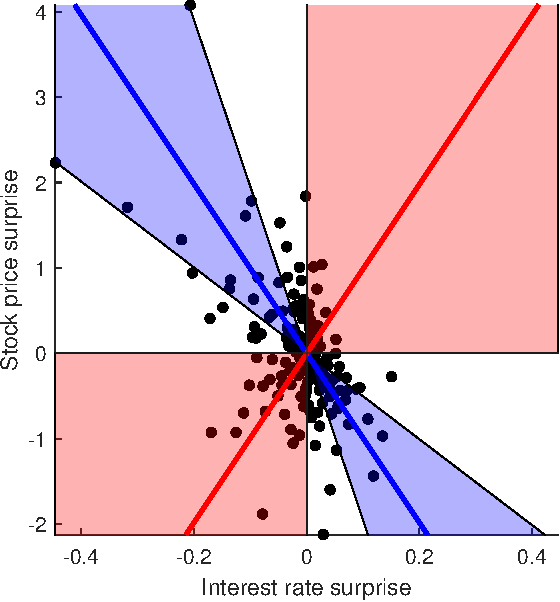
\includegraphics[width=0.45\textwidth]{figures/fed-scatter-rotations}&
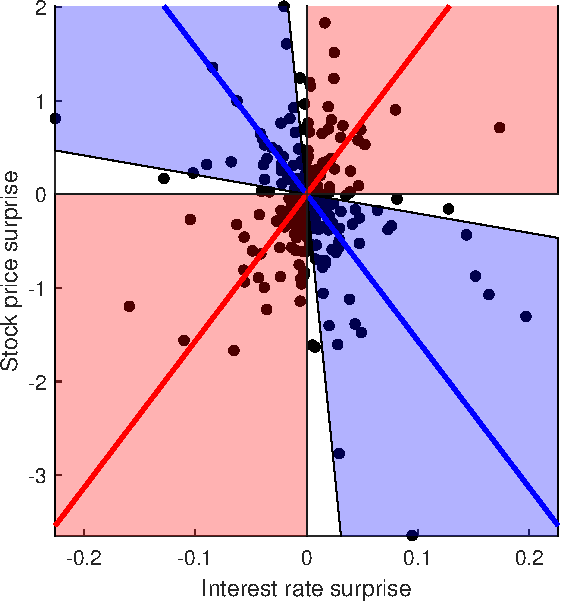
\includegraphics[width=0.45\textwidth]{figures/ecb-scatter-rotations}\\
Fed announcements & ECB announcements
\end{tabular}
\end{center}
\footnotesize Note. Each dot corresponds to one announcement. In each plot, the blue line represents the relationship $s = c_{MP}* i^{MP}$ and the red line represents the relationship 
$s = c_{CBI}* i^{CBI}$ for the median rotation. Blue and red ranges represent the slopes of these relations for all the admissible decompositions.
\end{figure}

Figure \ref{fig: rotation extremes} reports the surprises and the admissible range of decompositions.
The scatter plots show the interest rate surprises and stock price
surprises for all Fed and ECB announcements.
The blue regions indicate all the admissible negative relations between $i^{Total}$ and $s$ conditionally on
the monetary policy shock, i.e. all the admissible lines  $s = c_{MP}\,i^{MP}$. 
The red regions indicate all the corresponding positive relations between $i^{Total}$ and $s$ conditionally on
the central bank shock, i.e. all the admissible lines  $s = c_{CBI}\,i^{CBI}$. 

\begin{table}[!htbp]
\begin{center}
\caption{Coefficients $c_{MP}$ and $c_{CBI}$ and variance shares corresponding to selected rotations}\label{tab: rotations}
\begin{tabular}{lccccccc}
\toprule
Percentile of the   & \multicolumn{3}{c}{Fed} & & \multicolumn{3}{c}{ECB}  \\
admissible rotations & $c_{MP}$ & $c_{CBI}$ & $\vsmp$ & & $c_{MP}$ & $c_{CBI}$ & $\vsmp$\\
\midrule
00th & -5.0 & $\infty$ & 1.00 &   & -2.1 & $\infty$ & 1.00 \\
25th & -7.3 & 27.1 & 0.93 &   & -7.9 & 39.3 & 0.88 \\
50th & -9.9 & 9.9 & 0.75 &   &-15.7 & 15.7 & 0.57 \\
75th & -13.5 & 3.6 & 0.51 &   &-31.1 & 6.3 & 0.22 \\
100th & -19.5 & 0.0 & 0.26 &   & -118.8 & 0.0 & 0.02 \\
\bottomrule
\end{tabular}
\end{center}
\end{table}

Table \ref{tab: rotations} reports the coefficients $c_{MP},c_{CBI}$ and variance shares $\vsmp$ for selected rotations. 
Smaller rotation angles produce $i^{MP}$ shocks that affect stock price surprises less and account for a higher share of variance of $i^{Total}$.
For both the ECB and the Fed the smallest admissible rotation angle corresponds to the recursive decomposition and implies that all interest rate surprises are interpreted as monetary policy shocks $i^{MP}$ (and the unexplained variation in stock price surprises is attributed to the `FOMC risk shock' as in \citealt{Kroencke_etal_2021}).

\section{Local projection results}

\subsection{Additional local projection results}

\renewcommand\textfraction{.02}
%%%%%%%%%%%%%%%%%%%%%%%%%% ECB surprises

\begin{table}[!htbp]
\begin{center}
\caption{The effect of ECB interest rate surprises and shocks on financial variables}\label{tab: reg ecb surp}
$y^{}_{t+h}-y^{}_{t-1} = \alpha + \beta_h\, i^{Total,ECB}_t + u_t.$\\
$y^{}_{t+h}-y^{}_{t-1} = \alpha + \beta^{MP}_h\, i^{MP}_t + \beta^{CBI}_h\, i^{CBI}_t + u_t.$
\small
\resizebox{0.95\textwidth}{!}{
\begin{tabular}{lcccccccccc} \toprule
 & $h=1$ & $h=2$ & $h=3$ & $h=4$ & $h=5$ & $h=10$ & $h=15$ & $h=20$ & $h=25$ & $h=30$
\input{\pathTables table-ecbsurp1a.txt}\\[-0.9cm]
\input{\pathTables table-ecbsurp1b.txt}
\tabularnewline\bottomrule
\end{tabular}}
\end{center}\footnotesize
Notes: Heteroskedasticity robust standard errors in parentheses. *** p$<$0.01, ** p$<$0.05, * p$<$0.1.
Constant terms are not reported for brevity.
\end{table}

%%%%%%%%%%%%%%%%%%%%%%%%%% ECB shocks: Fed funds futures


\begin{table}[!htbp]\small
\begin{center}
\caption{The effect of ECB monetary policy and information shocks on Fed funds futures, omitting the Zero Lower Bound period.}\label{tab: lp ecb shocks fff nozlb}
\resizebox{\textwidth}{!}{
\begin{tabular}{lcccccccccc} \toprule
 & $h=1$ & $h=2$ & $h=3$ & $h=4$ & $h=5$ & $h=10$ & $h=15$ & $h=20$ & $h=25$ & $h=30$
\input{\pathTables table-ecbshocks4.txt}
\tabularnewline\bottomrule
\end{tabular}
}
\end{center}
Notes: Heteroskedasticity robust standard errors in parentheses. *** p$<$0.01, ** p$<$0.05, * p$<$0.1.
Constant terms are not reported for brevity.
Ftest: p-value of the F-test for H0: $\beta^{MP}_h=\beta^{CBI}_h$.
The sample excludes the period between 16 December 2008 and 15 December 2015, when the Fed funds rate was stuck near zero.
\end{table}

\clearpage

\subsection{Local projection results corresponding to the figures in the text}

%%%%%%%%%%%%%%%%%%%%%%%%%% ECB shocks
\begin{table}[!htbp]
\begin{center}
\caption{The effect of ECB monetary policy and information shocks on financial variables}\label{tab: lp ecb shocks}
$y^{}_{t+h}-y^{}_{t-1} = \alpha + \beta^{MP}_h\, i^{MP}_t + \beta^{CBI}_h\, i^{CBI}_t + u_t.$
\small
\resizebox{\textwidth}{!}{
\begin{tabular}{lcccccccccc} \toprule
 & $h=1$ & $h=2$ & $h=3$ & $h=4$ & $h=5$ & $h=10$ & $h=15$ & $h=20$ & $h=25$ & $h=30$
\input{\pathTables table-ecbshocks2.txt}
\tabularnewline\bottomrule
\end{tabular}}
\end{center}\footnotesize
Notes: Heteroskedasticity robust standard errors in parentheses. *** p$<$0.01, ** p$<$0.05, * p$<$0.1.
Constant terms are not reported for brevity.
Ftest: p-value of the F-test for H0: $\beta^{MP}_h=\beta^{CBI}_h$.
\end{table}


\begin{table}[!htbp]\addtocounter{table}{-1}\small
\begin{center}
\caption{Continued}
\resizebox{\textwidth}{!}{
\begin{tabular}{lcccccccccc} \toprule
 & $h=1$ & $h=2$ & $h=3$ & $h=4$ & $h=5$ & $h=10$ & $h=15$ & $h=20$ & $h=25$ & $h=30$
\input{\pathTables table-ecbshocks3.txt}
\tabularnewline\bottomrule
\end{tabular}}
\end{center}\footnotesize
Notes: Heteroskedasticity robust standard errors in parentheses. *** p$<$0.01, ** p$<$0.05, * p$<$0.1.
Constant terms are not reported for brevity.
Ftest: p-value of the F-test for H0: $\beta^{MP}_h=\beta^{CBI}_h$.
\end{table}


%%%%%%%%%%%%%%%%%%%%%%%%%% EA macro surprises

\begin{table}[!htbp]
\begin{center}
\caption{The effect of European industrial confidence surprises on financial variables}\label{tab: lp z ea bcs confind}
$y^{}_{t+h}-y^{}_{t-1} = \alpha + \beta_h\, z^{IndConf}_t + u_t$
\small
\resizebox{0.97\textwidth}{!}{
\begin{tabular}{lcccccccccc} \toprule
 & $h=1$ & $h=2$ & $h=3$ & $h=4$ & $h=5$ & $h=10$ & $h=15$ & $h=20$ & $h=25$ & $h=30$
\input{\pathTables table-z_ea_bcs_confind.txt}
\tabularnewline\bottomrule
\end{tabular}}
\end{center}\footnotesize
Notes: Heteroskedasticity robust standard errors in parentheses. *** p$<$0.01, ** p$<$0.05, * p$<$0.1.
Constant terms are not reported for brevity.
\end{table}

\begin{table}[!htbp]
\begin{center}
\caption{The effect of euro area unemployment rate surprises on financial variables}\label{tab: lp z ea unemp}
$y^{}_{t+h}-y^{}_{t-1} = \alpha + \beta_h\, z^{Unemp}_t + u_t$
\small
\resizebox{0.97\textwidth}{!}{
\begin{tabular}{lcccccccccc} \toprule
 & $h=1$ & $h=2$ & $h=3$ & $h=4$ & $h=5$ & $h=10$ & $h=15$ & $h=20$ & $h=25$ & $h=30$
\input{\pathTables table-z_ea_unemp.txt}
\tabularnewline\bottomrule
\end{tabular}}
\end{center}\footnotesize
Notes: Heteroskedasticity robust standard errors in parentheses. *** p$<$0.01, ** p$<$0.05, * p$<$0.1.
Constant terms are not reported for brevity.
\end{table}

%%%%%%%%%%%%%%%%%%%%%%%%%% ECB shocks: Stocks

\begin{table}[!htbp]\small
\begin{center}
\caption{The effect of ECB monetary policy and information shocks on stock sub-indices.}\label{tab: lp ecb shocks stocks}
\resizebox{\textwidth}{!}{
\begin{tabular}{lcccccccccc} \toprule
 & $h=1$ & $h=2$ & $h=3$ & $h=4$ & $h=5$ & $h=10$ & $h=15$ & $h=20$ & $h=25$ & $h=30$
\input{\pathTables table-ecbshocks-stocks1.txt}
\tabularnewline\bottomrule
\end{tabular}
}
\end{center}
Notes: Heteroskedasticity robust standard errors in parentheses. *** p$<$0.01, ** p$<$0.05, * p$<$0.1.
Constant terms are not reported for brevity.
Ftest: p-value of the F-test for H0: $\beta^{MP}_h=\beta^{CBI}_h$.
\end{table}

\begin{table}[!htbp]\addtocounter{table}{-1}\small
\begin{center}
\caption{Continued}
\resizebox{\textwidth}{!}{
\begin{tabular}{lcccccccccc} \toprule
 & $h=1$ & $h=2$ & $h=3$ & $h=4$ & $h=5$ & $h=10$ & $h=15$ & $h=20$ & $h=25$ & $h=30$
\input{\pathTables table-ecbshocks-stocks2.txt}
\tabularnewline\bottomrule
\end{tabular}}
\end{center}
Notes: Heteroskedasticity robust standard errors in parentheses. *** p$<$0.01, ** p$<$0.05, * p$<$0.1.
Constant terms are not reported for brevity.
Ftest: p-value of the F-test for H0: $\beta^{MP}_h=\beta^{CBI}_h$.
\end{table}

\begin{table}[!htbp]\addtocounter{table}{-1}\small
\begin{center}
\caption{Continued}
\resizebox{\textwidth}{!}{
\begin{tabular}{lcccccccccc} \toprule
 & $h=1$ & $h=2$ & $h=3$ & $h=4$ & $h=5$ & $h=10$ & $h=15$ & $h=20$ & $h=25$ & $h=30$
\input{\pathTables table-ecbshocks-stocks3.txt}
\tabularnewline\bottomrule
\end{tabular}}
\end{center}
Notes: Heteroskedasticity robust standard errors in parentheses. *** p$<$0.01, ** p$<$0.05, * p$<$0.1.
Constant terms are not reported for brevity.
Ftest: p-value of the F-test for H0: $\beta^{MP}_h=\beta^{CBI}_h$.
\end{table}

%%%%%%%%%%%%%%%%%%%%%%%%%% EA macro surprises - stocks

\begin{table}[!htbp]
\begin{center}
\caption{The effect of European industrial confidence surprises on stock sub-indices}\label{tab: lp z ea bcs confind stocks}
$y^{}_{t+h}-y^{}_{t-1} = \alpha + \beta_h\, z^{IndConf}_t + u_t$
\small
\resizebox{0.97\textwidth}{!}{
\begin{tabular}{lcccccccccc} \toprule
 & $h=1$ & $h=2$ & $h=3$ & $h=4$ & $h=5$ & $h=10$ & $h=15$ & $h=20$ & $h=25$ & $h=30$
\input{\pathTables table-z_ea_bcs_confind-stocks.txt}
\tabularnewline\bottomrule
\end{tabular}}
\end{center}\footnotesize
Notes: Heteroskedasticity robust standard errors in parentheses. *** p$<$0.01, ** p$<$0.05, * p$<$0.1.
Constant terms are not reported for brevity.
\end{table}

\begin{table}[!htbp]
\begin{center}
\caption{The effect of euro area unemployment rate surprises on stock sub-indices}\label{tab: lp z ea unemp stocks}
$y^{}_{t+h}-y^{}_{t-1} = \alpha + \beta_h\, z^{Unemp}_t + u_t$
\small
\resizebox{0.97\textwidth}{!}{
\begin{tabular}{lcccccccccc} \toprule
 & $h=1$ & $h=2$ & $h=3$ & $h=4$ & $h=5$ & $h=10$ & $h=15$ & $h=20$ & $h=25$ & $h=30$
\input{\pathTables table-z_ea_unemp-stocks.txt}
\tabularnewline\bottomrule
\end{tabular}}
\end{center}\footnotesize
Notes: Heteroskedasticity robust standard errors in parentheses. *** p$<$0.01, ** p$<$0.05, * p$<$0.1.
Constant terms are not reported for brevity.
\end{table}


%%%%%%%%%%%%%%%%%%%%%%%%%% Fed shocks

\begin{table}[!htbp]
\begin{center}
\caption{The effect of Fed monetary policy and information shocks on financial variables}\label{tab: reg fed shocks}
$y^{}_{t+h}-y^{}_{t-1} = \alpha + \beta^{MP}_h\, i^{MP}_t + \beta^{CBI}_h\, i^{CBI}_t + u_t.$
\small
\resizebox{\textwidth}{!}{
\begin{tabular}{lcccccccccc} \toprule
 & $h=1$ & $h=2$ & $h=3$ & $h=4$ & $h=5$ & $h=10$ & $h=15$ & $h=20$ & $h=25$ & $h=30$
\input{\pathTables table-fedshocks1.txt}
\tabularnewline\bottomrule
\end{tabular}}
\end{center}\footnotesize
Notes: Heteroskedasticity robust standard errors in parentheses. *** p$<$0.01, ** p$<$0.05, * p$<$0.1.
Constant terms are not reported for brevity.
Ftest: p-value of the F-test for H0: $\beta^{MP}_h=\beta^{CBI}_h$.
\end{table}

\begin{table}[!htbp]\addtocounter{table}{-1}\small
\begin{center}
\caption{Continued}
\resizebox{\textwidth}{!}{
\begin{tabular}{lcccccccccc} \toprule
 & $h=1$ & $h=2$ & $h=3$ & $h=4$ & $h=5$ & $h=10$ & $h=15$ & $h=20$ & $h=25$ & $h=30$
\input{\pathTables table-fedshocks2.txt}
\tabularnewline\bottomrule
\end{tabular}}
\end{center}\footnotesize
Notes: Heteroskedasticity robust standard errors in parentheses. *** p$<$0.01, ** p$<$0.05, * p$<$0.1.
Constant terms are not reported for brevity.
Ftest: p-value of the F-test for H0: $\beta^{MP}_h=\beta^{CBI}_h$.
\end{table}


\clearpage

\section{Additional VAR results}\label{sec: app var}

\subsection{Simple (``poor man'') decomposition}

\begin{figure}[!htbp]
\caption{The effects of ECB shocks on the US variables: Impulse responses to one standard deviation  MP and CBI shocks obtained with the simple decomposition in monthly VARs.}\label{fig: var ecb shocks poorman}
\renewcommand{\pathFigures}{../workm_var/ecb/us_gdp_ecb_pm}
\newcommand{\myfig}[1]{\includegraphics[width=0.37\textwidth]{\pathFigures-#1}}
\begin{center}
\begin{tabular}{cc}
\myfig{sveny01_a}&
\myfig{sveny10_a}\\
\myfig{sp500_a}&
\myfig{bofaml_us_hyld_oas_a}\\
\myfig{eurusd_a}&
\myfig{broadexea_usd_a}\\
\myfig{us_rgdp}&
\myfig{us_gdpdef}\\
\end{tabular}
\end{center}
\footnotesize Note: The red solid-dotted lines represent the point-wise posterior medians of the impulse responses to the central bank information shock. The red areas show pointwise 16-84 percentile bands. 
The blue solid lines and blue areas show the same objects for the monetary policy shock. 
The figure is based on 10,000 draws from the Gibbs sampler.
\end{figure}

\subsection{Domestic effects of monetary policies}

\begin{figure}[!htbp]
\caption{The effects of ECB shocks on the euro area variables: Impulse responses to one standard deviation ``rotation-based''  MP and CBI shocks in monthly VARs.}\label{fig: var ecb shocks rotation domestic}
\renewcommand{\pathFigures}{../workm_var/ecb/ea_gdp_ecb_sgnm2}
\newcommand{\myfig}[1]{\includegraphics[width=0.35\textwidth]{\pathFigures-#1}}
\newcommand{\myfigx}[1]{\includegraphics[width=0.35\textwidth]{../workm_var/ecb/#1}}
\begin{center}
\begin{tabular}{cc}
\myfigx{ea_wx_ecb_sgnm2-ea_wuxia} & \myfigx{ea_kr_ecb_sgnm2-ea_krippner}\\
\myfig{bund1y_a} & \myfig{bund10y_a}\\
\myfig{stoxx50_a} & \myfig{bofaml_ea_hyld_oas_a}\\
\myfig{eurusd_a} & \myfig{broad_eur}\\
\myfig{ea_rgdp} & \myfig{ea_gdpdef}\\
\end{tabular}
\end{center}
\footnotesize Note: The red solid-dotted lines represent the point-wise posterior medians of the impulse responses to the central bank information shock. The red areas show pointwise 16-84 percentile bands. 
The blue solid lines and blue areas show the same objects for the monetary policy shock. 
The figure is based on 10,000 draws from the Gibbs sampler.
\end{figure}

\begin{figure}[!htbp]
\caption{The effects of Fed shocks on the US variables: Impulse responses to one standard deviation ``rotation-based''  MP and CBI shocks in monthly VARs.}\label{fig: var fed shocks rotation domestic}
\renewcommand{\pathFigures}{../workm_var/fed/us_gdp_fed_sgnm2}
\newcommand{\myfig}[1]{\includegraphics[width=0.35\textwidth]{\pathFigures-#1}}
\newcommand{\myfigx}[1]{\includegraphics[width=0.35\textwidth]{../workm_var/fed/#1}}
\begin{center}
\begin{tabular}{cc}
\myfigx{us_wx_fed_sgnm2-us_wuxia} & \myfigx{us_kr_fed_sgnm2-us_krippner}\\
\myfig{sveny01_a} & \myfig{sveny10_a}\\
\myfig{sp500_a} & \myfig{bofaml_us_hyld_oas_a}\\
\myfig{eurusd_a} & \myfig{broadexea_usd_a}\\
\myfig{us_rgdp} & \myfig{us_gdpdef}\\
\end{tabular}
\end{center}
\footnotesize Note: The red solid-dotted lines represent the point-wise posterior medians of the impulse responses to the central bank information shock. The red areas show pointwise 16-84 percentile bands. 
The blue solid lines and blue areas show the same objects for the monetary policy shock. 
The figure is based on 10,000 draws from the Gibbs sampler.
\end{figure}

\clearpage
\bibliographystyle{econ}
\bibliography{spillovers}

\end{document}
